

\chapter{Solving The Hubbard Model}




\section{Mean Field Equations}

\subsubsection{The Mean Field Hamiltonian}

We treat the Hubbard model in a perturbative approach at the mean field level.
The Hubbard term  $H_U$ represents the perturbation.
The two-particle operator can be written as a product of two single particle operators.
We can rewrite any product of two operators $\hat{A}$ and $\hat{B}$ as
\begin{IEEEeqnarray}{rCl}
 \hat{A}\cdot\hat{B} 
		    &=&	 \left(\hat A - \langle \hat A \rangle \right) \left( \hat B -\langle \hat B \rangle \right)
			 +\langle \hat A \rangle \hat B
			 +\langle \hat B \rangle \hat A
			 - \langle \hat A \rangle \langle \hat B \rangle
\end{IEEEeqnarray}
In the mean field approach we neglect the first term on the right hand side –the product of fluctuations around their expectation value– leaving us with
\begin{equation}
  \hat{A}\cdot\hat{B} 
		   \approx 
			 \langle \hat A \rangle \hat B
			 +\langle \hat B \rangle \hat A 
			 - \langle \hat A \rangle \langle \hat B \rangle
\end{equation}
% RPA has nothing to do with this I think…
%
We use this relation on the single particle operators 
$c^{\dagger}_{\vec k,\uparrow}c_{\vec k - \vec q,\uparrow}$
and 
$c^{\dagger}_{\vec k,\downarrow}c_{\vec k + \vec q,\downarrow}$
in the Hubbard term of the Hamiltonian. 
Furthermore, we drop the constant term corresponding to $\langle \hat A \rangle \langle \hat B \rangle$, since a constant in the Hamiltonian will not have any
influence on the dynamics of the system. 
The mean field approximation of the Hubbard term reads
\begin{equation}
 H_U \stackrel{\mathrm{mf}}{\approx}  \frac{U}{N}
 \sum_{\vec{q}} \sum_{\sigma} 
 \left( \sum_{\vec{p}^{\prime}} \langle c^{\dagger}_{\vec{p}^{\prime},-\sigma} c_{\vec{p}^{\prime}+\vec{q},-\sigma} \rangle \right)
	\sum_{\vec p}  c^{\dagger}_{\vec{p},\sigma} c_{\vec{p}-\vec{q},\sigma}. \label{Hubbard_mean_field}
\end{equation}
The expectation value for the one particle operator is different from zero for only two values of $\vec q$.
First, for $\vec q = 0$ the expression yields the spin dependent filling factor, i.e. the number of particles with spin $\sigma$ relative to the total number of sites $N$.
\begin{equation}
 n_{\sigma} = \frac1N \sum_{\vec k} \langle c^{\dagger}_{\vec k, \sigma} c_{\vec k, \sigma} \rangle.
\end{equation}
A single  site can be empty or occupied by one particle at a given spin $\sigma$. The possible values for $n_{\sigma}$ are therefore restricted to the range $[0,1]$.
The total number density is simply the sum of both spin dependent number densities, $n=n_{\uparrow}+n_{\downarrow}$ 
and ranges from the empty case $n=0$ to 2, corresponding to a situation where each site is occupied by two particles with opposite spin.


The second contribution comes from $\vec q = (\frac12, \frac12)$ in units of $\frac{2\pi}a$, which we will use as the momentum unit throughout the whole thesis.
This vector acts as a nesting vector $\vec Q$ for the Fermi surface of the band structure. 
This means that large parts of the Fermi surface can be mapped onto itself by a translation of this vector. 

The dispersion of a square lattice with only nearest-neighbour interactions 
 %can be divided into two sublattices $A$ and $B$, 
 %such that hopping occurs only from one sublattice to the other.
%and as a 
%The partition in sublattices can be understood as an enlargement of the unit cell, resulting in a reduced Brillouin zone of half the size.
%At the same time, we have now to energy disperions, belonging to each sublattice. 
%
depends only on $\cos(k_x) + \cos(k_y)$.
and is therefore perfectly nested.
That means
$\varepsilon_{\vec k} = -\varepsilon_{\vec k + \vec Q}$.
The Fermi surface at half filling is in this case a perfect square.
Introducing higher order hopping terms deforms the Fermi surface, but nesting with $\vec Q$ holds on a approximate level for small $t^{\prime}$ and $t^{\prime \prime}$.
The Fermi surfaces together with the nesting vector $\vec Q$ are shown for both cases in figure \ref{fig:energie_dispersion}.
%
%
%
%$\vec Q$ is the basis vector for antiferromagnetic ordering. 
%This is observed in these materials \todo{how general, which ones} and expected % for what reason?


Nesting with $\vec Q = (\frac 12, \frac12)$ leads to a non-zero expectation value for $\langle c^{\dagger}_{\vec k, \sigma} c_{\vec k + \vec Q ,\sigma} \rangle $
and therefore to a symmetry broken ground state with an anti-ferromagnetic moment. 
The staggered magnetization is the order parameter of an anti-ferromagnetic state. It counts spins with an alternating sign for each lattice site. 
It is maximized for a perfect distribution of alternating spins. 
Using $\euler^{\vec Q \vec R_i} = (-1)^i$ we can write the expectation value of the staggered magnetization 
in momentum space,
\begin{IEEEeqnarray}{lCl}
 m_{s} &=& m_{s, \uparrow} - m_{s, \downarrow}, \\
 m_{s, \sigma} &=& \frac1N  \sum_i (-1)^i \langle c^{\dagger}_{i,\sigma} c_{i,\sigma} \nonumber \\ &=&
 \frac1N \sum_{\vec k} \langle c^{\dagger}_{\vec k , \sigma} c_{\vec k + \vec Q, \sigma} \rangle .
\end{IEEEeqnarray}


In terms of the above defined parameters equation \ref{Hubbard_mean_field} simplifies finally to
\begin{equation}
 \hat H = \sum_{\vec k, \sigma} \left( \varepsilon_{\vec k } - \mu + U n_{-\sigma} \right) c^{\dagger}_{\vec k, \sigma} c_{\vec k ,\sigma}
	  + U m_{s,-\sigma} \sum_{\vec k, \sigma} c^{\dagger}_{\vec k + \vec Q, \sigma} c_{\vec k, \sigma}.
\end{equation}
%
%\begin{equation}
% H_U \approx \sum_{\sigma} \left( U n_{-\sigma} \sum_{\vec{p}} c^{\dagger}_{\vec{p}, \sigma} c_{\vec p, \sigma} 
%	      + \frac{ U m_{s,-\sigma}}2
%			      \sum_{\vec p} \left(  c^{\dagger}_{\vec{p}+\vec Q, \sigma} c_{\vec p, \sigma} 
%	                                          + c^{\dagger}_{\vec{p}       , \sigma} c_{\vec p+ \vec Q, \sigma} \right) \right)
%\end{equation}
%
%\begin{IEEEeqnarray}{rCl}
% H_{\mathrm{mf}} &=
%		\sum_{\vec{p},\sigma} &
%				      \left( \varepsilon_{\vec k} - \mu + U n_{-\sigma} \right) 
%					  c^{\dagger}_{\vec{p},\sigma} c_{\vec{p},\sigma}
%				      +\frac{U}2  m_{s,-\sigma}	 
%					  \left( c^{\dagger}_{\vec{p}+\vec{Q},\sigma} c_{\vec{p},\sigma} +\mathrm{h.c.} %c^{\dagger}_{\vec{p},\sigma} c_{\vec{p}+\vec{Q},\sigma} 
%					  \right)					 
%\end{IEEEeqnarray}
%
We are left with a Hamilton operator consisting only of single particle operators. 
That shows the idea of the mean field approach, describing non-interacting particles that are exposed to an averaged field.
This field is the result off the sum of all particles in the system. It's value will therefore be influenced by the particles itself.
As a result we have to solve the equations for the fields self-consistently, which will be done in the next section. 
The first term in the above mean field Hamiltonian represents the mean repulsion due to the equal charge of the electrons.
The strength of the repulsion seen by a particle with a certain spin is proportional to the number density of particles with the opposite spin,
since the on-site interaction couples only particles with different spin. 

The second term corresponds to the coupling to a staggered magnetic field, that is a magnetic field with an alternating orientation on each site. 
The field strength is proportional to the magnetization of the ground state and given by $Um_s$.

\subsubsection{Mean Field Propagators}

The mean field Hamiltonian gives rise to two different propagators.
First we get the diagonal contribution, second an off-diagonal one from the staggered component. 
The propagators are defined by
\begin{IEEEeqnarray}{rCl}
 G_{\vec k}(\tau) &=& -\langle \mathcal{T}_{\tau} c_{\vec k         ,\sigma}(\tau)  c^{\dagger}_{\vec k ,\sigma}(0) \rangle \\
 F_{\vec k}(\tau) &=& -\langle \mathcal{T}_{\tau} c_{\vec k +\vec{Q},\sigma}(\tau)  c^{\dagger}_{\vec k ,\sigma}(0) \rangle \label{Def_Propagator}
\end{IEEEeqnarray}
with the imaginary time ordering operator $\mathcal{T}_{\tau}$, acting on a pair of fermion operators according to
\begin{IEEEeqnarray}{rCl}
 \mathcal{T}_{\tau} \hat{A}(\tau_1) \hat{B}(\tau_2) &=&
 -\Theta(\tau_1-\tau_2)\hat{A}(\tau_1) \hat{B}(\tau_2) + \Theta(\tau_2-\tau_1)\hat{B}(\tau_2) \hat{A}(\tau_1) \nonumber \\
 &=& \left\{ \begin{array}{r@{\text{ for }}l} -\hat{A}(\tau_1) \hat{B}(\tau_2) & \tau_1 \ge \tau_2 \\ \hat{B}(\tau_2) \hat{A}(\tau_1) & \tau_1 < \tau_2 \end{array} \right.
\end{IEEEeqnarray}
%
From this definition it follows that $n_\sigma$ and $m_{s,\sigma}$ can be expressed in terms of propagators, namely through
\begin{IEEEeqnarray}{lCl}
 n_{\sigma} &=& \frac1N \sum_{\vec k} \left( 1-G_{\vec k, -\sigma}(0) \right) \label{n_DEF}\\
 m_{s,\sigma} &=& -\frac1N \sum_{\vec k} F_{\vec k, -\sigma}(0)		\label{m_DEF}
\end{IEEEeqnarray}


The equation of motion for operators, $\frac{\dint}{\dint \tau} \hat{A} = [H,\hat{A}] + \frac{\partial}{\partial_{\tau}} \hat{A}$,
determines the dependence of the propagators on imaginary time. 
Using the definition of propagators in Eq. (\ref{Def_Propagator})  and the equation of motion,
we get the differential equation.
\begin{IEEEeqnarray}{rCl}
 \partial_{\tau} G_{\vec k ,\sigma}(\tau) 
 &=&
 \delta(\tau) \langle c_{\vec k ,\sigma}(\tau) c^{\dagger}_{\vec k ,\sigma}(0) + c^{\dagger}_{\vec k ,\sigma}(0) c_{\vec k ,\sigma}(\tau) \rangle \nonumber \\&&
 + \Theta(\tau) \langle [\hat H , c_{\vec k ,\sigma}(\tau)] c^{\dagger}_{ \vec k ,\sigma}(0) \rangle		\nonumber \\ &&
 -  \Theta(-\tau) \langle c^{\dagger}_{ \vec k ,\sigma}(0) [\hat H , c_{\vec k ,\sigma}(\tau)]  \rangle \label{EOM_G}
\end{IEEEeqnarray}
Here we used $\partial_{\tau} \Theta(\tau) = \delta(\tau)$.
The commutators can be evaluated using the identity $[AB,C] = A\{B,C\} - \{A,C\}B$ and the anti-commutation rules for the creation and annihilation operators in
equation \ref{acomm_rules}.
%
This results in
\begin{equation}
 [H,c_{\vec k ,\sigma}(\tau)]=-\left(\varepsilon_{\vec k}-\mu + Un_{-\sigma} \right) c_{\vec k ,\sigma}(\tau) - Um_{s,-\sigma} c_{\vec k +\vec{Q},\sigma}(\tau)
\end{equation}
Putting this back in equation (\ref{EOM_G}) together with the definitions for $G$ and $F$, we get
\begin{IEEEeqnarray}{rCl}
  \partial_{\tau} G_{\vec k ,\sigma}(\tau) 
&=&
\delta(\tau)\langle \{c_{\vec k ,\sigma}(\tau),c^{\dagger}_{\vec k ,\sigma}(0)\} \rangle
- \left( \varepsilon_{\vec k }-\mu+ Un_{-\sigma} \right) G_{\vec k ,\sigma}(\tau)  \nonumber \\ &&
 -Um_{s,-\sigma} F_{\vec k ,\sigma}(\tau) \label{EOM_G_II}
\end{IEEEeqnarray}
In the next step we take the Fourier transform of this equation. 
The Fourier transformed propagator is related to the propagator in imaginary time through
\begin{IEEEeqnarray}{rCl}
 G_{\vec k ,\sigma}(\tau) &=& \frac{1}{\beta} \sum_n \euler^{-\im \omega_n \tau} G_{\vec k ,\sigma}(\im \omega_n) \\
 G_{\vec k ,\sigma}(\im \omega_n) &=& \int_0^{\beta} \! \!\dint  \tau \: \euler^{\im \omega_n \tau} G_{\vec k ,\sigma}(\tau)
\end{IEEEeqnarray}
The so called fermionic Matsubara frequencies $\omega_n$ are given by $\omega_n = \frac{\pi}{\beta}(2n+1), \; n \! \in \! \mathbb{Z}$.
By this definition, the fermionic Greens's functions are anti-periodic with respect to shifts in $\tau$ by $\beta$, $G(\tau+\beta) = -G(\tau)$.
Transforming equation (\ref{EOM_G_II}) to momentum space we get
\begin{IEEEeqnarray}{rCl}
 \left( \im \omega_n -\varepsilon_{\vec k } +\mu - Un_{-\sigma} \right) G_{\vec k ,\sigma}(\im \omega_n) = 1 +Um_{s,-\sigma} F_{\vec k ,\sigma}(\im \omega_n)
\end{IEEEeqnarray}
In the same way, starting from $\frac{\dint}{\dint \tau} F_{\vec k ,\sigma}(\tau)$ we get for the off-diagonal propagator
\begin{IEEEeqnarray}{rCl}
 \left( \im \omega_n -\varepsilon_{\vec k +\vec{Q}} +\mu - Un_{-\sigma} \right) F_{\vec k ,\sigma}(\im \omega_n) = Um_{s,-\sigma} G_{\vec k ,\sigma}(\im \omega_n)
\end{IEEEeqnarray}
There is no constant term, since the anti-commutator in \ref{EOM_G_II} is zero for off-diagonal momenta. 
Putting the last two equations together we get the expressions for the propagators
\begin{IEEEeqnarray}{rCl}
 G_{\vec k ,\sigma}(\im \omega_n) &=& \frac{ ( \im \omega_n - \varepsilon_{\vec k +\vec{Q}} + \mu -Un_{-\sigma} )}
			      { ( \im \omega_n - \varepsilon_{\vec k +\vec{Q}} + \mu -Un_{-\sigma} )
			        ( \im \omega_n - \varepsilon_{\vec k }         + \mu -Un_{-\sigma} )
			      - U^2m_{s,-\sigma}^2 } \nonumber \\
			      &&\nonumber  \\ && \\
 F_{\vec k ,\sigma}(\im \omega_n) &=& \frac{ Um_{s,-\sigma}}
			    { ( \im \omega_n - \varepsilon_{\vec k +\vec{Q}} + \mu -Un_{-\sigma} )
			      ( \im \omega_n - \varepsilon_{\vec k }         + \mu -Un_{-\sigma} )
			      - U^2m_{s,-\sigma}^2 }			\nonumber      
\end{IEEEeqnarray}
We can rewrite this in a more appealing way by factorizing the denominator of both propagators. 
The poles are located at
\begin{equation}
 E_{\vec k ,\sigma}^{\pm}
 =
 \frac{\varepsilon_{\vec k }+\varepsilon_{\vec k +\vec{Q}}}2 -\mu + Un_{-\sigma}  \pm \sqrt{ \left(\frac{\varepsilon_{\vec k }-\varepsilon_{\vec k +\vec{Q}}}2\right)^2 + U^2m_{s,-\sigma}^2 }
 \label{EpmDef}
\end{equation}
Note that $E_{\vec k ,\sigma}^{\pm}=E_{\vec k +\vec{Q},\sigma}^{\pm}$, since $\varepsilon_{\vec k +2\vec{Q}}=\varepsilon_{\vec k }$.
These energies correspond to the formation of two bands, defined over the reduced or magnetic Brillouin zone.
The antiferromagnetic ordering loweres the symmetry of the crystal, and enlarges therfore the unit cell.
At the same time the Brillouin zone is reduced, which explains the periodicity in $\vec Q$. 
The band structure is shown in figure \ref{EpmDisp}. 
\begin{figure}
 \begin{center}
  \includegraphics[width=.9\textwidth]{../EpEm_tttU44}
  \caption{$E^+_{\vec k}$ and $E^-_{\vec k}$ band for $U=4.4$ and $(t,t^{\prime},t^{\prime \prime})=(1.0,0.22,0.12)$ in dimensionless units.}
\label{EpmDisp}
  \end{center}
 \end{figure}
%
It can be seen clearly, that the bands are well separated.
It is conclusive form their expression, that the bands are separated by approximately $Um_s$ for large enough $U$.
The split up is a result of the repulsive interaction and the symmetry breaking of the anti-ferromagnet ground state.
The $J=\frac12$-band is half filled, the lower of the split bands $E^-_{\vec k}$ is therefore fully occupied, while 
$E^+_{\vec k}$ is remains empty. 
This makes Sr$_2$IrO$_4$ an insulator.
This only possible since, because the $t_{2g}$ states were already split into two smaller bands by the strong SOC.
Changing the parameters for SOC and electron-electron repulsion a little changes the situation significantly.
Sr$_2$RhO$_4$, which  is equal to Sr$_2$IrO$_4$ in structure and electron configuration,
just with the $4d$ orbital is metallic\cite{PhysRevLett.96.246402}. 
The interaction in the $4d$ orbitals is stronger, while at the same time the SOC is to weak, to create the same bands 
as in the Ir case. The interaction is then not strong enough, to split the rather broad $t_{2g}$ band.
As a result Sr$_2$RhO$_4$ is a paramagnetic metal.
This shows the importance of strong SOC for the properties of Sr$_2$IrO$_4$. 
%
It further supports  the statement, that Sr$_2$IrO$_4$  experiences the effects of both types of mechanisms to create insulators,
the charge interaction driven Mott type and the Slater type, which is based on magnetic ordering \cite{PhysRevB.89.165115},
since its and gap depends on the repulsion as well as the antiferromagnetic ordering.


%The transition from a Mott insulator to a paramagnetic metal is dependent on the strength of the SOC. 
%With $\lambda = 1.1t$ the critical value of a multi orbit model is $U_c=3.3t$ \cite{PhysRevLett.105.216410}, Sr$_2$IrO$_4$ is therefore 
%in the  anti-ferromagnetic phase, but close to the metal insulator transition. 
%Using Rh instead of Ir increases $U$, but reduces $\lambda$ at the same time. 
%A larger $U$ on the one hand increases the band gap, with a low lambda however we do not necessarily have the 
%effective spin-$\frac12$ states anymore. 




Using the expressions for the energies $E^{\pm}_{\vec k}$, the propagators can be expressed in terms of the new bands,
\begin{IEEEeqnarray}{rCl}
 G_{\vec k ,\sigma}(\im \omega_n) &=& \frac{ \im \omega_n - \varepsilon_{\vec k +\vec{Q}} +\mu -Un_{-\sigma} }
					    { (\im \omega_n - E_{\vec k ,\sigma}^+) (\im \omega_n - E_{\vec k ,\sigma}^-) },
\\
 F_{\vec k ,\sigma}(\im \omega_n) &=& \frac{ Um_{s,-\sigma} }
					    { (\im \omega_n - E_{\vec k ,\sigma}^+) (\im \omega_n - E_{\vec k ,\sigma}^-)}.
\end{IEEEeqnarray}
We note that $F_{\vec k,\sigma}$ is invariant under a translation $\vec k \rightarrow \vec k +\vec Q$, 
while $G_{\vec k,\sigma}$ changes depending on the dispersion $\varepsilon_{\vec k}$.


%\begin{IEEEeqnarray}{rCl}
%  G_{\vec{p},\sigma}(\im \omega_n) &=& \frac{ u_{\vec{p}        ,\sigma }}{ (\im \omega_n - E_{\vec{p},\sigma}^+) }
%			+ \frac{ u_{\vec{p}+\vec{Q},\sigma }}{ (\im \omega_n - E_{\vec{p},\sigma}^-) } \\
%  F_{\vec{p},\sigma}(\im \omega_n) &=& \frac{ \tilde{u}_{\vec{p},\sigma }}{ (\im \omega_n - E_{\vec{p},\sigma}^+) }
%			- \frac{ \tilde{u}_{\vec{p},\sigma }}{ (\im \omega_n - E_{\vec{p},\sigma}^-) }
%\end{IEEEeqnarray}
%where $u$ and $\tilde{u}$ are given by
% \begin{IEEEeqnarray}{rCl}
% u_{\vec{p},\sigma} &=& \frac{E_{\vec{p},\sigma}^+ - \varepsilon_{\vec{p}+\vec{Q}} +\mu -Un_{-\sigma} }{E_{\vec{p},\sigma}^+ -E_{\vec{p},\sigma}^-} \\
% \tilde{u}_{\vec{p},\sigma} &=& \frac{Um_{s,-\sigma}}{E_{\vec{p},\sigma}^+ -E_{\vec{p},\sigma}^-}.
% \end{IEEEeqnarray}
% \todo{connection to diagrammatic approach, resolve $1-n_{-\sigma} \stackrel{?}{=} n_{-\sigma}$ issue.} 
% \todo{ How to draw nice diagrams in \LaTeX?}

There is an alternative approach from a diagrammatic point of view, that gives the same differential equation for the propagators.
Following the notation of \cite{PhysRevB.65.132404}, 
we denote the bare propagator $G^0_{\vec k,\sigma}$ by a single line, the mean field propagators by double lines and the interaction by a dashed line.
The off-diagonal propagator $F_{\vec k ,\sigma}$ is marked with an doubled arrow head.
The diagrams for a self-consistent mean field approximation are shown in figure \ref{Diagr_Props}. 


\begin{fmffile}{prop}

\fmfcmd{%
style_def dbl_plain_dbl_arrow expr p =
draw_double p;
shrink(1.5);
cfill (harrow (p, 0.8));
cfill (harrow (p, 0.7));
endshrink;
enddef;}

\begin{figure}
 \begin{center}
 \begin{IEEEeqnarray}{rCl}
%\vcenter{ \hbox{
 \parbox{20mm}{
	      \begin{fmfgraph}(20mm,30mm)
		\fmfleft{i1}
		\fmfright{o1}
		\fmf{dbl_plain_arrow}{i1,o1}
	      \end{fmfgraph}}
&=& \parbox[][][t]{15mm}{\begin{fmfgraph}(15mm,30mm) \fmfleft{i} \fmfright{o} \fmf{plain_arrow}{i,o} \end{fmfgraph}} 
   + \parbox{25mm}{\begin{fmfgraph}(25mm,30mm) \fmfleft{i1} \fmfright{o1} \fmf{plain_arrow}{i1,v1} \fmf{dbl_plain_dbl_arrow}{v1,o1}
					   \fmf{dashes,tension=0}{v2,v1} 	 \fmfforce{0.5w,.8h}{v2}     \fmf{dbl_plain_dbl_arrow,tension=0.3}{v2,v2}
                \end{fmfgraph}}
	+    \parbox{25mm}{\begin{fmfgraph}(25mm,30mm) \fmfleft{i1} \fmfright{o1} \fmf{plain_arrow}{i1,v1} \fmf{dbl_plain_arrow}{v1,o1}
					   \fmf{dashes,tension=0}{v2,v1} 	 \fmfforce{0.5w,.8h}{v2}     \fmf{dbl_plain_arrow}{v2,v2} \end{fmfgraph}}
 \end{IEEEeqnarray}
 \begin{IEEEeqnarray}{rCl}
 \parbox{20mm}{
	      \begin{fmfgraph}(20mm,30mm)
		\fmfleft{i1}
		\fmfright{o1}
		\fmf{dbl_plain_dbl_arrow}{i1,o1}
	      \end{fmfgraph}}
&=& \parbox{25mm}{\begin{fmfgraph}(25mm,30mm) \fmfleft{i1} \fmfright{o1} \fmf{dbl_plain_dbl_arrow}{i1,v1} \fmf{plain_arrow}{v1,o1}
					   \fmf{dashes,tension=0}{v2,v1} 	 \fmfforce{0.5w,.8h}{v2}     \fmf{dbl_plain_arrow}{v2,v2}
                \end{fmfgraph}}
	+    \parbox{25mm}{\begin{fmfgraph}(25mm,30mm) \fmfleft{i1} \fmfright{o1} \fmf{plain_arrow}{i1,v1} \fmf{dbl_plain_arrow}{v1,o1}
					   \fmf{dashes,tension=0}{v2,v1} 	 \fmfforce{0.5w,.8h}{v2}     \fmf{dbl_plain_dbl_arrow}{v2,v2} \end{fmfgraph}}
\end{IEEEeqnarray} 
\end{center}
\caption{Self consistent mean field equations for $G_{\vec k, \sigma}$ and $F_{\vec k, \sigma}$.}
\label{Diagr_Props}
\end{figure} 
% 
%
By including only single loops we neglect again the possibility of quantum fluctuations, i.e. there are no interactions with virtual states.
Note that the particles on each site of the interaction have different spins and there is no spin transfer. 
All straight arrows have therefore the same spin, while the propagators forming the loops have the opposite spin.
We reflect the sum up to infinite such interactions by using the mean field propagator after the interaction. 
%
Self-consistency is achieved by using the mean field propagators in the loops.
This reflects the fact, that $m_{s,\sigma}$ and $n_{\sigma}$ itself depend on the sum over the respective mean field propagator.
As a result we have to solve the equations for $m_{s,\sigma}$ and $n_{\sigma}$ iteratively. % CHECK IF THIS SENTENCE APPEARS LATER AGAIN.
%
Inserting the bare propagator ${G^0_{\vec k,\sigma}(\im \omega_n)}=(\im \omega_n +\varepsilon_{\vec k} - \mu)^{-1}$ of the non interacting system
as well as equations \ref{n_DEF} and \ref{m_DEF}
reproduces the above expressions for $G_{\vec k, \sigma}$ and $F_{\vec k ,\sigma}$.






%\subsubsection{Validity of mean field Description}
% This should maybe be the first point in the mean field section
%In order to treat the Hubbard model in the mean field approach we rely on assumptions. that limit this approach to a certain set of parameters.
% Antiferromagnetic groundstate – low T
% low fluctuations
% Mott insulator
% effect of quantum fluctuations





\section{Observables}

In the chapters above we derived an effective Hamiltonian for the iridates.
Furthermore we introduced the Green's functions of the mean field approach. 
We can use this formalism now, to calculate observable quantities.
They can be compared to experiments to validate the calculations. 
The interaction parameter $U$ has to be fitted to experiments as well.



\subsubsection{X-Ray and Neutron Scattering Experiments}

The main experimental techniques that resolve the magnetic structure of such materials are inelastic neutron and x-ray scattering experiments.
Neutrons are uncharged and do therefore not  interact with the charges of atoms and electrons in the crystal.
This allows them to penetrate thick probes and to interact well below the surface, which makes measurements of the bulk possible. 
They interact solely through their intrinsic spin with the crystal, 
which makes them good candidates for probing the magnetic excitation spectrum.

During the last two decades, resonant inelastic x-ray scattering (RIXS) became an important alternative.
It uses high energetic photons, whose energy is tuned to be resonant to an atomic transition in the system.
The exited electron is lifted in the bands at the Fermi level, where they can interact with particles close to this band.
When the whole created by the incident photon is filled with some electron from that band, a secondary photon is sent out. 
The secondary photon might have a different energy and momentum due to the dynamics of particles in the relevant band,
which is the reason, that this process is inelastic.


In both cases, neutron and photon scattering,  we can measure the momentum transfer and energy transfer to the probe.
The differential cross section $\frac{\dint^2 \sigma}{\dint \Omega \dint \omega}$ is the distribution of secondary particles with a certain momenta. 
The difference to the momenta of the primary photon is passed to the probe as an excitation.
At basic excitations of the system scattering becomes resonant and the differential cross section has a pole.
The position $(\vec q, \omega)$ of these  poles reveal therefore the  dispersion of magnetic excitations in the material.

The differential cross section is proportional to the imaginary part of the retarded response function \cite[Chapter~7.3.1]{altland2010condensed},
which will be described in the next paragraph. 
\begin{equation}
 \frac{\dint^2 \sigma}{\dint \Omega \dint \omega} = -2 \Im \left( \chi(\omega \vec q) \right)
\end{equation}


\subsubsection{Response Functions}

Response functions describe the reaction of the system to an external distortion.
The distortion is some generalized external force $F$, for example an electromagnetic field.
This force might vary in space and time.
It needs to be coupled to the system through some sort of interaction, that is introduced into the Hamiltonian by a additional term 
$\hat H_F = \hat X(F)$ 
for some operator $\hat X$.
In the simplest case, $X$ is linear in $F$, that is $X = X^{\prime} F$.
A linear dependence provides a good description for week perturbations of the system, that is for $F\rightarrow 0$.
$X^{\prime}$ is then just the first term of an expansion of $X$. 
%
The effect on the system will then be measured by the change in some observable $y=\langle Y \rangle$,
which might coincide with the operator $X^{\prime}$.
%
The response of the system is then completely encoded in the linear response function $\chi$, which depends in $Y$ and $X^{\prime}$, 
but is  independent of the external force $F$.


The dynamic magnetic susceptibility is the linear response function to an external space and time dependent magnetic field $\vec B(\vec r,t)$.
It couples to the  magnetic moment $\vec M$ in the system through $  \int \dint^3 r \hat{\vec M}(\vec r) \vec B(\vec r,t)$.
The distortion is quantified through $ \vec M$ as well.
The magnetic susceptibility is therefore proportional to the expectation value of magnetic structure factor. 
\begin{equation}
\chi^{ab}(\vec q,\omega) = \int \dint \tau \euler^{\im \omega \tau} \langle  M^a(q,\tau) M^b(-\vec q, 0) \rangle 
\end{equation}
Measurements are often performed on a poly-crystals or powder. 
Therefore we don't have a fixed crystal orientation, but rather an average over all spatial orientations.
The effective susceptibility is therefore diagonal with the components
\begin{equation}
 \chi^{ab}_{\mathrm{eff}} = \delta^{ab} \mathrm{Tr}(\chi) = \delta^{ab} \langle \vec M(q,\tau) \vec M(-\vec q, 0) \rangle \label{magnSuscI}
\end{equation}



In the simplest case, the spin axes are parallel to the symmetry axes of the crystal.
$\vec M$ is then proportional to the spin $\vec J$. 
The spin operator is a one-particle operator with the components $a=x,y,z$, defined as
\begin{equation}
 J^a(R_i)= J^a_i = \frac12\sum_{\sigma,\sigma^{\prime}} c^{\dagger}_{i,\sigma} \left(\sigma^a \right)_{\sigma\sigma^{\prime}} c_{i,\sigma},
\end{equation}
$\sigma^a$ are the Pauli matrices.
%
The momentum space  representation is
\begin{IEEEeqnarray}{rCl}
J^{a}(\vec q) &=& \frac12\sum_{i} \sum_{\sigma,\sigma^{\prime}}  \euler^{\im \vec q \vec R_i} c^{\dagger}_{i ,\sigma} \left(\sigma^a \right)_{\sigma\sigma^{\prime}} c_{i} \nonumber \\
&=& \frac12\sum_{\vec k} \sum_{\sigma,\sigma^{\prime}} c^{\dagger}_{\vec k, \sigma} \left(\sigma^a \right)_{\sigma\sigma^{\prime}} c_{\vec k + \vec q,\sigma^{\prime}}
\end{IEEEeqnarray}
%

In Sr$_2$IrO$_4$ it is the field of the ligands, that define the spin axes. 
The octahedra are rotated by $\pm \Theta$ in the $x$-$y$-plane in a staggered pattern.
It is therefore necessary, to project the spin components on the axes of the lattice at each site.
The relation between the magnetic moment, expressed in the axis of thelattice, and the spin $\vec J_i$  at site $i$ is therefore 
related by a space dependent coordinate transformation.
The transformation matrix  at site $i$ is
\begin{equation}
 \vec M_i = \left( \begin{array}{ccc} \cos(\Theta) & -(-1)^i \sin(\Theta) & 0 \\ (-1)^i \sin(\Theta) & \cos(\Theta) & 0 \\ 0&0&1 \end{array} \right) \vec J_i
\end{equation}
This transformation can lead to a small ferromagnetic moment in an antiferromagnetic ground state.
If we describe the antiferromagnetic ordering with respect to the $x$-axis of the spins,
then we get a net magnetization in $y$-direction, since the alternating sign in the transformation matrix cancels the spin flip in 
the antiferromagnetic ordering.
\begin{figure}
 \begin{center}
  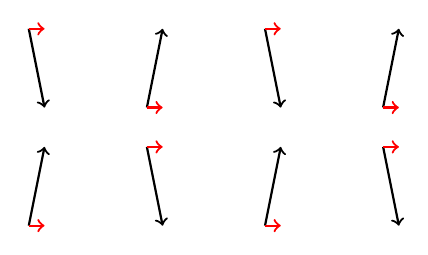
\begin{tikzpicture}
   \draw[->,thick] (-0.1,0) -- (+0.1,1);
   \draw[->,red,thick] (-0.1,0) -- (+0.1,0);
   \draw[<-,thick] (1.6,0) -- (1.4,1);
   \draw[->,red,thick] (1.4,1) -- (+1.6,1);
   \draw[->,thick] (2.9,0) -- (3.1,1);
   \draw[->,red,thick] (2.9,0) -- (3.1,0);
   \draw[<-,thick] (4.6,0) -- (4.4,1);
   \draw[->,red,thick] (4.4,1) -- (4.6,1);
  %
   \draw[<-,thick] (+0.1,1.5) -- (-0.1,2.5);
   \draw[->,red,thick] (-0.1,2.5) -- (+0.1,2.5);
   \draw[->,thick] (1.4,1.5) -- (1.6,2.5);
   \draw[->,red,thick] (1.4,1.5) -- (1.6,1.5);
   \draw[<-,thick] (3.1,1.5) -- (2.9,2.5);
   \draw[->,red,thick] (2.9,2.5) -- (3.1,2.5);
   \draw[->,thick] (4.4,1.5) -- (4.6,2.5);
   \draw[->,red,thick] (4.4,1.5) -- (4.6,1.5);
   \end{tikzpicture}
 \end{center}
\caption{The staggered rotation of antiferromagnetic spins lead to a net ferromagnetic moment (red)}
\label{mFerr}
\end{figure}

The ferromagnetic moment is proportional to the antiferromagnetic ordering times the projected component,
\begin{equation}
 m = \sin \Theta m_s.
\end{equation}



The alternating sign $(-1)^i$ in the rotations express the staggered pattern and
can be expressed through the wave vector of antiferromagnetic ordering $\vec Q$, 
which reads $(-1)^i = \euler^{\im \vec Q \vec R_i}$.
In momentum space, the relation between magnetic moment and spin is therefore
\begin{equation}
 \left( \begin{array}{c} M^x_{\vec q} \\ M^y_{\vec q} \\ M^z_{\vec q} \end{array} \right) = 
-2\mu_b \left( \begin{array}{c} \cos(\Theta) J^x_{\vec q} -\sin(\Theta) J^y_{\vec q + \vec Q} \\ \cos(\Theta) J^y_{\vec q} +\sin(\Theta) J^x_{\vec q + \vec Q} \\ J^z_{\vec q} \end{array} \right) 
\end{equation}






We can replace $\vec M$ in equation \ref{magnSuscI} and get
\begin{IEEEeqnarray}{rCl}
 \chi_{\mathrm{eff}}(\omega,\vec q) &=& \cos^2{\Theta} \left( \chi_J^{xx}(\omega,\vec q)+ \chi_J^{yy}(\omega,\vec q) \right) \nonumber \\ &&
 + \sin^2\Theta \left(\chi_J^{xx} (\omega, \vec q + \vec Q) + \chi_J^{yy}(\omega,\vec p + \vec Q)\right)
 + \chi_J^{zz}
\end{IEEEeqnarray}
Where we introduced the spin susceptibility $\chi_J^{ab}(\tau,\vec q = \langle J^a(\tau,\vec q) J^b(0,\vec q) \rangle$. 
Based on the transformation of Pauli matrices $\sigma^{\pm} = \sigma^x \pm \im \sigma^y$ we get the spin components $J^{\pm}$, 
which fulfil the relation $J^{\pm} = (J^{\mp})^{\dagger}$.
Using this relation we can express the sum of $xx$ and $yy$ components of the spin susceptibility in terms of $+-$ and $-+$ components,
\begin{equation}
 \chi_J^{xx} + \chi_J^{yy} = \chi_J^{+-} + \chi_J^{-+} = 2\chi_J^{+-}
\end{equation}
The magnetic susceptibility gets therefore the form
\begin{equation}
 \chi_{\mathrm{eff}}(\omega, \vec q) = 2\cos^2\Theta \chi_J^{+-}(\omega,\vec q)  + 2\sin^2\Theta\chi_J^{+-}(\omega,\vec q+ \vec Q) + \chi_J^{zz}(\omega, \vec q)
\end{equation}


\subsection{Dynamic Magnetic Susceptibility In The Green's Function Formalism}


We can expand the spin susceptibility in terms of Green's functions. 
We will first calculate the transverse susceptibility $\chi_J^{+-}$, by summing up the relevant diagrams.
The longitudinal component $\chi_J^{zz}$ is then calculated in a similar manner.


%The components of the magnetic susceptibility are defined by
%\begin{equation}
% \chi^{ab}(\tau - \tau^{\prime}) = \sum_{\vec{p}} \left( \sum_{\alpha, \beta} c^{\dagger}_{\vec k, \alpha }(\tau) \left(\sigma^{a}\right)_{\alpha \beta} c_{\vec k , \beta}(\tau)  \right)
%			    \cdot \left(  \sum_{\gamma, \delta} c^{\dagger}_{\vec k, \gamma }(\tau^{\prime}) \left(\sigma^{b}\right)_{\gamma \delta} c_{\vec k , \delta}(\tau^{\prime}) \right)  
%\end{equation}


Expressing $\chi_J^{+-}$ and $\chi_J^{-+}$ in creation and destruction operators gives
\begin{IEEEeqnarray}{rCl}
 \chi^{+-}(\vec q,\omega) &=& \int_0^{\beta} \!\!\dint \tau \euler^{\im \omega \tau} \langle \mathcal{T}_{\tau} S^+(\vec q,\tau) S^-(-\vec q,0) \rangle \nonumber \\
			  &=&\int_0^{\beta} \!\!\dint \tau \euler^{\im \omega \tau} 
			  \sum_{\vec k \vec k^{\prime}} \langle c^{\dagger}_{\vec k,\downarrow}(\tau) c_{\vec k+\vec q, \uparrow}(\tau) 
								    c^{\dagger}_{\vec k^{\prime}+\vec q,\downarrow}(0) c_{\vec k^{\prime},\uparrow}(0) \rangle.
\end{IEEEeqnarray}
As a four point correlation function, it describes the propagation of a particle-hole pair with momentum $\vec q$.
We restrict the sum over all diagrams to the most relevant subclass.
It is given by diagrams, which form a chain of bubbles or a ladder of particle-hole pairs.
This approximation is known as the random phase approximation (RPA). 
Since the particle and hole propagator of such basic excitations are always connected at the same vertices, their product is independent of the phase. 
This would not be the case if interactions with quantum fluctuations were taken into account. 
The situation corresponds to a phase that  is randomly distributed and cancels therefore in the 
thermodynamic limit. 
Those are furthermore the diagrams, where each occurrence of $\frac UN$ is paired with a sum over momenta, which runs over all $N$ momenta.
Diagrams beyond the RPA have fewer integrations over free momenta and are therefore suppressed in the large N limit.
The first order bubble diagrams of the RPA expansion are shown in figure \ref{1orderLadder}.
%
%
\begin{figure}
\centering
\begin{tabular}{cc}
 \begin{fmfgraph*}(120,45)
  \fmfleft{i1} \fmfright{o1} \fmf{dots_arrow,tension=2,label=$\vec q$}{i1,v1} \fmf{dbl_plain_arrow,left=.35}{v1,v2,v4} 
  \fmf{dbl_plain_arrow,left=.35}{v4,v3,v1} \fmf{dots_arrow,tension=2,label=$\vec q$}{v4,o1}
  \fmfforce{.5w,h}{v2} \fmfforce{.5w,0}{v3} \fmf{dashes,tension=0}{v2,v3}
 \end{fmfgraph*}
 &
% \begin{fmfgraph*}(120,45)
%  \fmfleft{i1} \fmfright{o1} \fmf{dots_arrow,tension=2,label=$\vec q$}{i1,v1} \fmf{dbl_plain_arrow,left=.35}{v1,v2,v4} 
%  \fmf{dbl_plain_arrow,left=.35}{v4,v3,v1} \fmf{dots_arrow,tension=2,label=$\vec q$}{v4,o1}
%  \fmfforce{.5w,h}{v2} \fmfforce{.5w,0}{v3} \fmf{dashes,tension=0}{v2,v3}
% \end{fmfgraph*}
% &
% \begin{fmfgraph*}(120,45)
%  \fmfleft{i1} \fmfright{o1} \fmf{dots_arrow,tension=2,label=$\vec q$}{i1,v1} \fmf{dbl_plain_arrow,left=.35}{v1,v2,v4} 
%  \fmf{dbl_plain_arrow,left=.35}{v4,v3,v1} \fmf{dots_arrow,tension=2,label=$\vec q$}{v4,o1}
%  \fmfforce{.5w,h}{v2} \fmfforce{.5w,0}{v3} \fmf{dashes,tension=0}{v2,v3}
% \end{fmfgraph*}
% \\
 \begin{fmfgraph*}(120,45)
  \fmfleft{i1} \fmfright{o1} \fmf{dots_arrow,tension=2,label=$\vec q$}{i1,v1} \fmf{dbl_plain_dbl_arrow,left=.35}{v1,v2,v4} 
  \fmf{dbl_plain_dbl_arrow,left=.35}{v4,v3,v1} \fmf{dots_arrow,tension=2,label=$\vec q$}{v4,o1}
  \fmfforce{.5w,h}{v2} \fmfforce{.5w,0}{v3} \fmf{dashes,tension=0}{v2,v3}
 \end{fmfgraph*}
 \\
 %\begin{fmfgraph*}(120,45)
 % \fmfleft{i1} \fmfright{o1} \fmf{dots_arrow,tension=2,label=$\vec q$}{i1,v1} \fmf{dbl_plain_arrow,left=.35}{v1,v2,v4} 
%  \fmf{dbl_plain_arrow,left=.35}{v4,v3,v1} \fmf{dots_arrow,tension=2,label=$\vec q$}{v4,o1}
%  \fmfforce{.5w,h}{v2} \fmfforce{.5w,0}{v3} \fmf{dashes,tension=0}{v2,v3}
% \end{fmfgraph*}
% &
 \begin{fmfgraph*}(120,45)
  \fmfleft{i1} \fmfright{o1} \fmf{dots_arrow,tension=2,label=$\vec q$}{i1,v1} \fmf{dbl_plain_arrow,left=.35}{v1,v2} \fmf{dbl_plain_dbl_arrow,left=.35}{v2,v4} 
  \fmf{dbl_plain_arrow,left=.35}{v4,v3} \fmf{dbl_plain_dbl_arrow,left=.35}{v3,v1} \fmf{dots_arrow,tension=2,label=$\vec q$}{v4,o1}
  \fmfforce{.5w,h}{v2} \fmfforce{.5w,0}{v3} \fmf{dashes,tension=0}{v2,v3}
 \end{fmfgraph*}
 &
 \begin{fmfgraph*}(120,45)
  \fmfleft{i1} \fmfright{o1} \fmf{dots_arrow,tension=2,label=$\vec q$}{i1,v1} \fmf{dbl_plain_arrow,left=.35}{v1,v2,v4} 
  \fmf{dbl_plain_dbl_arrow,left=.35}{v4,v3,v1} \fmf{dots_arrow,tension=2,label=$\vec q$}{v4,o1}
  \fmfforce{.5w,h}{v2} \fmfforce{.5w,0}{v3} \fmf{dashes,tension=0}{v2,v3}
 \end{fmfgraph*}
% &
% \begin{fmfgraph*}(120,45)
%  \fmfleft{i1} \fmfright{o1} \fmf{dots_arrow,tension=2,label=$\vec q$}{i1,v1} \fmf{dbl_plain_dbl_arrow,left=.35}{v1,v2,v4} 
%  \fmf{dbl_plain_arrow,left=.35}{v4,v3,v1} \fmf{dots_arrow,tension=2,label=$\vec q$}{v4,o1}
%  \fmfforce{.5w,h}{v2} \fmfforce{.5w,0}{v3} \fmf{dashes,tension=0}{v2,v3}
% \end{fmfgraph*} &
 \end{tabular}
 \caption{some of the first order diagrams contributing to $\chi^{+-}(\vec q, \im \omega_n)$.}
 \label{1orderLadder}
\end{figure}
%
%
Each step in the ladder consists a product of two propagators, which can be the diagonal one $G_{\vec q, \sigma}$
or the off-diagonal propagator $F_{\vec q, \sigma}$, as well as the interaction term $\frac{U}{N}$ times a delta function. 
The building blocks for the ladder diagrams are listed in table \ref{blocks}.
%
%
\begin{table}
\centering
\begin{tabular}{|c|V|c|}
\hline &&\\[.0cm]
 $\lambda$ &  
 \begin{fmfgraph}(60,35)
  \fmfleft{i1,i2} \fmfright{o1,o2}  \fmf{dashes,tension=0}{i1,i2} \fmf{phantom}{i1,o1} \fmf{phantom}{i2,o2} \fmfdot{i1,i2}
 \end{fmfgraph}
 & $\frac UN\delta(\vec k_1-\vec k_2 + \vec k_3 - \vec k_4)$  \\[.8cm]
 %
 $\lambda x$ & 
\begin{fmfgraph*}(60,35)
  \fmfleft{i1,i2} \fmfright{o1,o2}  \fmf{dashes,tension=0}{i1,i2} \fmf{dbl_plain_arrow}{o1,i1} \fmf{dbl_plain_arrow}{i2,o2} \fmfdot{i1,i2,o1,o2}
  \fmfv{l=$\uparrow$,l.a=25,l.d=1}{o1}
  \fmfv{l=$\downarrow$,l.a=-25,l.d=1}{o2}
 \end{fmfgraph*}
 & $\frac UN\sum_{\vec k,n^{\prime}} G_{\vec k, \downarrow}(\im \omega_{n^{\prime}}) G_{\vec k +\vec q,\uparrow }(\im \omega_{n^{\prime}} + \im \omega_n)$ \\[.8cm]
 %
 $\lambda y$ &
\begin{fmfgraph*}(60,35)
  \fmfleft{i1,i2} \fmfright{o1,o2}  \fmf{dashes,tension=0}{i1,i2} \fmf{dbl_plain_dbl_arrow}{o1,i1} \fmf{dbl_plain_dbl_arrow}{i2,o2}
  \fmfv{l=$\uparrow$,l.a=25,l.d=1}{o1}
  \fmfv{l=$\downarrow$,l.a=-25,l.d=1}{o2}
  \fmfdot{i1,i2,o1,o2}
 \end{fmfgraph*} 
 & $\frac UN\sum_{\vec k,n^{\prime}} F_{\vec k, \downarrow}(\im \omega_{n^{\prime}}) F_{\vec k +\vec q,\uparrow }(\im \omega_{n^{\prime}} + \im \omega_n)$ \\[.8cm]
 %
 $\lambda z_1$ &
 \begin{fmfgraph*}(60,35)
  \fmfleft{i1,i2} \fmfright{o1,o2}  \fmf{dashes,tension=0}{i1,i2} \fmf{dbl_plain_dbl_arrow}{o1,i1} \fmf{dbl_plain_arrow}{i2,o2}
    \fmfv{l=$\uparrow$,l.a=25,l.d=1}{o1}
  \fmfv{l=$\downarrow$,l.a=-25,l.d=1}{o2}
  \fmfdot{i1,i2,o1,o2}
 \end{fmfgraph*}
 &  $\frac UN\sum_{\vec k,n^{\prime}} G_{\vec k, \downarrow}(\im \omega_{n^{\prime}}) F_{\vec k +\vec q,\uparrow }(\im \omega_{n^{\prime}} + \im \omega_n)$ \\[.8cm]
 %
 $\lambda z_2$ &
 \begin{fmfgraph*}(60,35)
  \fmfleft{i1,i2} \fmfright{o1,o2}  \fmf{dashes,tension=0}{i1,i2} \fmf{dbl_plain_arrow}{o1,i1} \fmf{dbl_plain_dbl_arrow}{i2,o2}
   \fmfv{l=$\uparrow$,l.a=25,l.d=1}{o1}
  \fmfv{l=$\downarrow$,l.a=-25,l.d=1}{o2}
  \fmfdot{i1,i2,o1,o2}
 \end{fmfgraph*}
 &  $\frac UN\sum_{\vec k,n^{\prime}} F_{\vec k, \downarrow}(\im \omega_{n^{\prime}}) G_{\vec k +\vec q,\uparrow }(\im \omega_{n^{\prime}} + \im \omega_n)$ \\
 \hline
\end{tabular}
\caption{building blocks of ladder diagrams for $\chi^{+-}(\vec q, \im \omega_n)$}
\label{blocks}
\end{table}
%
Momentum conversation at each vertex limits the sum over momenta in each block to $\vec k^{\prime} = \vec k + \vec q$ or $\vec k^{\prime} = \vec k + \vec q + \vec Q$
The second possibility is due to the off-diagonal propagator $F_{\vec k,\sigma}$, that adds $\vec Q$ to the momentum. 
Each block consists of a sum over the Brillouin zone, we can therefore shift the momentum in the product of propagators without changing the value of the sum.
As mentioned above, only $G_{\vec k,\sigma}$ changes under a shift of $\vec Q$, $F_{\vec k,\sigma}$ however is invariant under such a transformation.
Therefore only $x$ will change it's value for $\vec q \rightarrow \vec q + \vec Q$, in all other situations the sum is unchanged, 
as the transformation can be absorbed in $F_{\vec k,\sigma}$,
We will write $\bar x$ to denote the expression for $x$ with $\vec k - \vec k^{\prime} = \vec q + \vec Q$.
When combining the building blocks of the ladder we have to keep track of the momentum difference $\vec k - \vec k^{\prime}$ in the sum over paired propagators.
In order to deal with the right momenta between upper and lower propagator we rewrite it as a $ 2 \times 2$ matrix equation and pick the value that 
corresponds to having $\vec q$ as the external momentum on both sides of the diagram.
The upper component in this matrix equation corresponds to $\vec k - \vec k^{\prime} = \vec q$, 
while the lower one corresponds to $\vec k -\vec k^{\prime} = \vec q + \vec Q$.
The full equation reads then
\begin{equation}
 \chi_{J}^{+-}(\vec q,\im \omega_n) = 
 \left( \begin{array}{cc} x+y & z_1+z_2 \end{array} \right) \cdot \sum_{m=0}^{\infty} (-\lambda \mathbf M)^m \cdot \left( \begin{array}{c} -1 \\  \: 0 \end{array} \right)
\end{equation}
with the matrix $\mathbf M$ combining all the possibilities for one new step in the ladder for each order $m$,
\begin{equation}\label{M_def}
\mathbf M =  \left( \begin{array}{cc} x+y & z_1+z_2 \\
			       z_1+ z_2 & \bar x +  y  \end{array} \right)
\end{equation}
At the end of a ladder diagram however we have to fulfil $\vec k - \vec k^{\prime} = \vec q$. 
The last vector ensures the right external momentum at the end and takes care of the minus sign, arising from the loop.
The infinite sum of bubble diagrams represents a geometric series and has an analytical expression.
Using the expression for geometric sums for matrices we can express the infinite sum through
\begin{IEEEeqnarray}{l}
 \sum_{m=0}^{\infty} (-\lambda \mathbf M)^m = \left( \mathbf{1} + \lambda \mathbf M \right)^{-1}  
 %\\ = \left[ \left(1+\lambda(x+y)\right)\left(1+\lambda(\bar x + \bar y)\right) - (z_1 +z_2)(\bar z_1 + \bar z_2) \right]^{-1} \left(\begin{array}{cc} 1+\lambda(\bar x+\bar y) & -(\bar z_1 + \bar z_2) \\ -(z_1 + z_2) & 1+\lambda(x+y) \end{array} \right) \nonumber
\end{IEEEeqnarray}
The whole expression reads then
\begin{equation}
 \chi_{\mathrm{RPA}}^{+-}(\vec q,\im \omega_n) = 
 \frac{ -(x+y)\left(1+\lambda(\bar x+ y) \right) +\lambda(z_1 + z_2)^2}
 {\left(1+\lambda(x+y)\right)\left(1+\lambda(\bar x + y)\right) - \lambda^2(z_1 +z_2)^2} \label{ladder_sum}
\end{equation}
In order to deal with the infinite Matsubara frequency summation we use the procedure from Appendix \ref{MFS},
as we did for finding $m_s$.
The remaining expression depends then only on $\im \omega_n$.
We are interested in the dependence on real frequencies $\omega$. 
Expression \ref{ladder_sum} possesses poles on the real axis, making a simple replacement of $\im \omega_ n$ with $\omega \in \mathbb{R}$ impossible. 
We perform the analytical continuation $\im \omega_n \rightarrow \omega + \im \eta$ with $\omega, \eta \in \mathbb{R}$ and for a small $\eta >0$.
By choosing $\eta$ to be positive we get the retarded response function. 
The expression can then be evaluated by carrying out the sum over the momenta using a small numerical value for $\eta$.
This allows us not only to calculate the imaginary part, a finite value of $\eta$ smoothes the resulting response function.
In general, for a function of the type $(\omega+\im \eta - E)^{-1}$, the imaginary part is 
$\frac{- \eta}{\eta^2 + (\omega-E)^2} \stackrel{\eta \rightarrow 0}{\longrightarrow} \pi \delta(\omega -E)$.
In the actual limit of vanishing $\eta$ we expect a delta function, whose poles might not match the discretized momenta of the grid exactly.
Broadening the delta function ensures to not miss momenta due to a finite sized grid and yields a result closer to actual measurements, 
where the response function also shows a finite line width. 

The position of the poles finally yields the spin-wave dispersion $\omega(\vec q)$.
Furthermore, we expect a continuum at higher energies. 

\subsubsection{Longitudinal Magnetic Susceptibility}

The longitudinal spin susceptibility consists of particle-hole propagators with equal spin.
This doesn't allow for interactions between particle and hole, but for recombination and creation of a new pair. 
The diagrams to be summed are therefore chains of bubbles.
\begin{figure}
\begin{tabular}{VV}
 \begin{fmfgraph*}(120,45)
  \fmfleft{i1} \fmfright{o1} 
  \fmf{dots_arrow,tension=1.0,label=$\vec q$}{i1,v1} 
  \fmf{dbl_plain_arrow,left=1.0,tension=.4}{v1,v2}
  \fmf{dbl_plain_arrow,left=1.0,tension=.4}{v2,v1}
  \fmf{dbl_plain_arrow,left=1.0,tension=0.4}{v4,v3} 
  \fmf{dbl_plain_arrow,left=1.0,tension=0.4}{v3,v4}
  \fmf{dots_arrow,tension=1.0,label=$\vec q$}{v4,o1}
  \fmf{dashes,tension=1.0}{v2,v3}
 \end{fmfgraph*}
 & 
  \begin{fmfgraph*}(120,45)
  \fmfleft{i1} \fmfright{o1} 
  \fmf{dots_arrow,tension=1.0,label=$\vec q$}{i1,v1} 
  \fmf{dbl_plain_dbl_arrow,left=1.0,tension=.4}{v1,v2}
  \fmf{dbl_plain_dbl_arrow,left=1.0,tension=.4}{v2,v1}
  \fmf{dbl_plain_dbl_arrow,left=1.0,tension=0.4}{v4,v3} 
  \fmf{dbl_plain_dbl_arrow,left=1.0,tension=0.4}{v3,v4}
  \fmf{dots_arrow,tension=1.0,label=$\vec q$}{v4,o1}
  \fmf{dashes,tension=1.0}{v2,v3}
 \end{fmfgraph*}
 \\
  \begin{fmfgraph*}(120,45)
  \fmfleft{i1} \fmfright{o1} 
  \fmf{dots_arrow,tension=1.0,label=$\vec q$}{i1,v1} 
  \fmf{dbl_plain_dbl_arrow,left=1.0,tension=.4}{v1,v2}
  \fmf{dbl_plain_dbl_arrow,left=1.0,tension=.4}{v2,v1}
  \fmf{dbl_plain_arrow,left=1.0,tension=0.4}{v4,v3} 
  \fmf{dbl_plain_arrow,left=1.0,tension=0.4}{v3,v4}
  \fmf{dots_arrow,tension=1.0,label=$\vec q$}{v4,o1}
  \fmf{dashes,tension=1.0}{v2,v3}
 \end{fmfgraph*}
 &
  \begin{fmfgraph*}(120,45)
  \fmfleft{i1} \fmfright{o1} 
  \fmf{dots_arrow,tension=1.0,label=$\vec q$}{i1,v1} 
  \fmf{dbl_plain_dbl_arrow,left=1.0,tension=.4}{v1,v2}
  \fmf{dbl_plain_arrow,left=1.0,tension=.4}{v2,v1}
  \fmf{dbl_plain_dbl_arrow,left=1.0,tension=0.4}{v4,v3} 
  \fmf{dbl_plain_arrow,left=1.0,tension=0.4}{v3,v4}
  \fmf{dots_arrow,tension=1.0,label=$\vec q$}{v4,o1}
  \fmf{dashes,tension=1.0,label=$\vec Q$}{v2,v3}
 \end{fmfgraph*}
 \end{tabular}
 \caption{some of the first order diagrams contributing to $\chi^{zz}$.}
 \label{bubbleex}
\end{figure}
%
Some exampled of the first order terms contributing to $\chi_J^{zz}$ are shown in figure \ref{bubbleex}.
Two consecutive bubbles must have opposite spin, so they can be connected by the interaction term.


\begin{table}
\centering
\begin{tabular}{|V|c|}
\hline &\\[.1cm]
%
\begin{fmfgraph*}(60,35)
  \fmfleft{i1} \fmfright{o1}  \fmf{dashes,tension=2.5}{i1,v1} \fmf{dbl_plain_arrow,left=1.00}{v1,o1} \fmf{dbl_plain_arrow,left=1.00}{o1,v1}
  \fmfv{l=$\sigma$,l.a=0,l.d=14}{v1}
  \fmfdot{i1,o1}
 \end{fmfgraph*}
 &$\lambda x$  or $\lambda \overline x $ \\[.8cm]
 %
\begin{fmfgraph*}(60,35)
  \fmfleft{i1} \fmfright{o1}  \fmf{dashes,tension=2.5}{i1,v1} \fmf{dbl_plain_dbl_arrow,left=1.00}{v1,o1} \fmf{dbl_plain_dbl_arrow,left=1.00}{o1,v1}
  \fmfv{l=$\sigma$,l.a=0,l.d=14}{v1}
 \fmfdot{i1,o1}
 \end{fmfgraph*}
 &$-\lambda y$ \\[.8cm]
 %
 \begin{fmfgraph*}(60,35)
  \fmfleft{i1} \fmfright{o1}  \fmf{dashes,tension=2.5}{i1,v1} \fmf{dbl_plain_dbl_arrow,left=1.00}{v1,o1} \fmf{dbl_plain_arrow,left=1.00}{o1,v1}
  \fmfv{l=$\sigma$,l.a=0,l.d=14}{v1}
  \fmfdot{i1,o1}
 \end{fmfgraph*}
 &$s_{\sigma}\lambda z_1$ \\[.8cm]
 %
 \begin{fmfgraph*}(60,35)
  \fmfleft{i1} \fmfright{o1}  \fmf{dashes,tension=2.5}{i1,v1} \fmf{dbl_plain_arrow,left=1.00}{v1,o1} \fmf{dbl_plain_dbl_arrow,left=1.00}{o1,v1}
  \fmfv{l=$\sigma$,l.a=0,l.d=14}{v1}
  \fmfdot{i1,o1}
 \end{fmfgraph*}
 &$-s_{\sigma}\lambda z_2$ \\[.8cm]
 %
 \hline
\end{tabular}
\caption{elements of the chain in $\chi_J^{zz}$}
\label{bubbles}
\end{table}
The bubbles in table \ref{bubbles} show the building blocks of the chains, that are summed up 
in the diagrammatic expansion of $\chi_J^{zz}$ in the random phase approximation. 
The second column shows the relation to the previously defined products of operators $x,y,z_1,z_2$.
Since only $F_{\vec k, \sigma}$ depends on the spin with the simple relation $F_{\vec k, -\sigma} = - F_{\vec k, \sigma}$,
the relation to the expressions found earlier is just a spin dependent sign.
Since the Hubbard interaction couples only spins with opposite orientation, two consecutive bubbles in the row must have opposite spin.
The last to blocks, proportional to $s_{\sigma}z_i$ change the momentum, that is transferred through the interaction by $\vec Q$. 
The difference of $\vec k$ and $\vec k^{\prime}$ between the upper and lower propagator in the bubble is therefore restricted to the external momentum $\vec q$ and 
a shifted momentum, $\vec q + \vec Q$.
In order to keep track of the alternating spins and the right transferred momentum, we set up a matrix as before. 
This time we have to deal with four components, that is spin and transferred vector. 
Let the components be $\left( (\vec q,\uparrow) , (\vec q+\vec Q,\uparrow) , (\vec q,\downarrow) , (\vec q+\vec Q,\downarrow) \right)^T$.
The sum over all possible chains can then be expressed as 
\begin{IEEEeqnarray}{rCl}
 \chi_J^{zz} &=& \langle \sum_{\vec k \vec k^{\prime}} 
 ( c^{\dagger}_{\vec k,\uparrow} c_{\vec k+\vec q,\uparrow} - c^{\dagger}_{\vec k,\downarrow} c_{\vec k+\vec q,\downarrow} )
 ( c^{\dagger}_{\vec k^{\prime},\uparrow} c_{\vec k^{\prime}+\vec q,\uparrow} - c^{\dagger}_{\vec k^{\prime},\downarrow} c_{\vec k^{\prime}+\vec q,\downarrow} ) \rangle
 \nonumber \\&=& 
   \left(\begin{array}{c}  x-y \\  z_1 -z_2 \\ y-x \\ z_1-z_2 \end{array} \right)^T  %\nonumber \\ &&  \quad \times 
\sum_{n=0}^{\infty}  (-\lambda)^n \left( \begin{array}{cc} 0 &  \mathbf M_{\downarrow} \\ \mathbf M_{\uparrow} & 0 \end{array} \right)^n 
 \left( \begin{array}{c} 1\\0\\-1\\0 \end{array}  \right) \label{zzDef}
\end{IEEEeqnarray}
The last vector ensures again that we pick the bubbles with $\vec k-\vec k^{\prime} = \vec q$ at the end of the chain.
The matrix $\mathbf M_{\sigma}$ is defined similar to $\mathbf M$ of equation \ref{M_def}. 
It differs only by the sign changes of it entries,
\begin{equation}
 \mathbf M_{\sigma} = \left( \begin{array}{cc} x-y & s_{\sigma}(z_1-z_2) \\ s_{\sigma} (z_1-z_2) & \overline x - y \end{array} \right) 
\end{equation}
The geometric sum can be regrouped in terms of even and odd powers of $n$.
After taking out one power from the odd sum we can add the two sums again and multiply it with unity plus on times the original matrix,
\begin{multline}
 \sum_n \lambda^n \left( \begin{array}{cc} 0 &  \mathbf M_{\downarrow} \\ \mathbf M_{\uparrow} & 0 \end{array} \right)^n  
 = 
\sum_n \lambda^{2n} \left( \begin{array}{cc}   \mathbf M_{\downarrow}\mathbf M_{\uparrow} & 0  \\ 0 & \mathbf M_{\uparrow}\mathbf M_{\downarrow}  \end{array} \right)^{2n} 
\left( \begin{array}{cc} 1 & -\lambda \mathbf M_{\uparrow} \\ \lambda -\mathbf M_{\downarrow} & 1 \end{array} \right) \\
=
\left( \begin{array}{cc}   (1-\lambda^2 \mathbf M_{\downarrow}\mathbf M_{\uparrow})^{-1}  & 0  \\ 0 & (1-\lambda^2 \mathbf M_{\uparrow}\mathbf M_{\downarrow})^{-1}  \end{array} \right)
\left( \begin{array}{cc} 1 & -\lambda \mathbf M_{\uparrow} \\ -\lambda \mathbf M_{\downarrow} & 1 \end{array} \right) 
 \end{multline}
Inserting the definition of $\mathbf M_{\sigma}$ in equation \ref{zzDef} and writing it out yields the closed form expression for
$\chi_J^{zz}$ in the random phase approximation,
\begin{multline}
 \chi_J^{zz} = 2 \Big( -(1-\lambda^2(\overline x-y)^2 + \lambda^2 (z_1-z_2)^2 ) (x-y) (1+\lambda(x-y)) \\
			+(1-\lambda^2( x-y)^2 + \lambda^2 (z_1-z_2)^2 ) \lambda (z_1-z_2) \\
	      + \lambda^2(x-\overline x)(z_1-z_2)^2 (1+2\lambda(x-y)) \Big) \\ 
			\times \left( \det(1-\mathbf M_{\uparrow} \mathbf M_{\downarrow} ) \right)^{-1}
\end{multline}
with the denominator
\begin{multline}
 \det(1-\mathbf M_{\uparrow} \mathbf M_{\downarrow} ) = \left((1-\lambda^2(x-y)^2 + \lambda^2(z_1-z_2)^2 \right) \\
		  \cdot \left(1-\lambda^2(\overline x-y)^2 + \lambda^2(z_1-z_2)^2 \right) \\
							  +\lambda^4(z_1-z_2)^2(x-\overline x)^2 
\end{multline}


 The expressions for $\chi_J^{+-}$ and $\chi_J^{zz}$ are imaginary through the use of imaginary frequencies in $x,y,z_1$ and $z_2$.
 We want to evaluate the expressions for real frequencies, but we have to keep an infinitesimal imaginary part due to poles on the 
 real frequency axis. This leads to a vanishing imaginary part, except for a vanishing denominator, where it resembles a delta function. 
 In order to find the poles it is therefore sufficient to evaluate the denominator to 0.

\end{fmffile}

\subsection{Corrections due to Quantum Fluctuations} \label{corrections}
  
The simplifications we made in order to treat the Hubbard model in the mean field approach,  
eliminate any effects that are caused by quantum fluctuations.
These effects may be small and we are able to cover the main features of the system with our simplified description,
but their effect have to be taken into account, especially when comparing calculations to measurements, where absolute values of observables are relevant.
One example is the staggered magnetization, that is overestimated in the mean field treatment. 
Fluctuations around the anti-ferromagnetic ground state act as a distortion to the ordering and lower therefore the expectation value of $m_s$.


Calculating the full corrections is beyond the scope of this thesis, but we can account for some major corrections, that have no complicated dependencies.
For the Heisenberg model, the corrections to the spin-wave-velocity, denoted by $\mathcal{Z}_c$, are well known.
They are given by the higher order terms of the $\frac1S$ expansion. 
The main contribution is independent of momentum and frequency. 
Higher order terms are an order of magnitude smaller and their momentum dependence changes the correction factor by $2\%$ at max.
Usually one uses therefore a constant of $\mathcal{Z}_c=1.18$ value to renormalize the whole spin-wave dispersion \cite{PhysRevB.45.10131}.

We will see that our calculation scheme provides the result of linear spin-wave theory without further corrections in the limit of large U. 
The Hubbard model can be expanded in this limit. The correction factor is the same as in the Heisenberg model, as one would except. 
In reference \cite{PhysRevB.43.3617}, Singh calculated corrections in the Hubbard model, 
given by diagrams corresponding to quantum fluctuations,
and found a value consistent with $\mathcal{Z}_c$.
We asume that the correction does not change substantially for smaller $U$ and correct $\omega$ in the expression for the dynamic magnetic susceptibility
by the constant $\mathcal Z_c = 1.18$.

% example of usage of Z_c in Heisenberg \cite{PhysRevB.43.3617}




% explain Z_c
% justify value, if needed from Singh
% staggered magnetization renormalization?

% what did we leave out:
% non-crossing approximation
% things that are not 1P-irreducible.

 